\documentclass{beamer}

\usepackage{import}
\usepackage{xifthen}
\usepackage{pdfpages}
% \usepackage{transparent}



% This file is a solution template for:

% - Talk at a conference/colloquium.
% - Talk length is about 20min.
% - Style is ornate.



% Copyright 2004 by Till Tantau <tantau@users.sourceforge.net>.
%
% In principle, this file can be redistributed and/or modified under
% the terms of the GNU Public License, version 2.
%
% However, this file is supposed to be a template to be modified
% for your own needs. For this reason, if you use this file as a
% template and not specifically distribute it as part of a another
% package/program, I grant the extra permission to freely copy and
% modify this file as you see fit and even to delete this copyright
% notice. 


\mode<presentation>
{
  \usetheme{Berlin}
  \setbeamercovered{transparent}
  \setbeamertemplate{caption}[numbered]
  \setbeamertemplate{footline}[frame number]
}


\usepackage[spanish,mexico]{babel}
% \usepackage[utf8]{inputenc}
\usepackage{times}
\usepackage[T1]{fontenc}

\title{Péndulo Simple}

\subtitle
{Modelado de sistemas}

\author[Equipo 1]{E. Benavides \and I. Ayala \and S. Campos \\ \and L. Almanza \and Y. Casas}


\institute[]
{
  Centro de Investigación y de Estudios Avanzados del IPN\\
  Robótica y Manufactura Avanzada
  }

\date[]{RyMA 2019}

\subject{System Modeling}



% Delete this, if you do not want the table of contents to pop up at
% the beginning of each subsection:
\AtBeginSubsection[]
{
  \begin{frame}<beamer>{Outline}
    \tableofcontents[currentsection,currentsubsection]
  \end{frame}
}


% If you wish to uncover everything in a step-wise fashion, uncomment
% the following command: 

%\beamerdefaultoverlayspecification{<+->}



\begin{document}

\begin{frame}
  \titlepage
\end{frame}

\begin{frame}{Contenido}
  \tableofcontents
\end{frame}

\section{Introducción}

\subsection{Objetivos}

\begin{frame}{Objetivos del proyecto}

  \begin{itemize}
    \item Desarrollar el modelo matemático del péndulo simple.
    \item Implementar un simulador del sistema en MATLAB.
    \item Comparar la simulación con un modelo físico.
  \end{itemize}
  
\end{frame}

\subsection{Trabajo previo}
\begin{frame}{Diagrama de cuerpo libre}
 \begin{figure}[ht]
    \centering
    \import{../Report/img/}{pendulum_diagram.pdf_tex}
    \caption{ Péndulo simple.}
    \label{fig: simple pendulum}
\end{figure}
\end{frame}

\begin{frame}{Mecánica Newtoniana y Lagrangiana}
\begin{itemize}
 \item Ecuación de movimiento para la formulación de Newton
 
 \begin{equation}
\ddot{\theta} = - \dfrac{g}{l} \sin(\theta) + \dfrac{k}{m} \dot{\theta}  
 \end{equation}

 \item Ecuación de movimiento para la formulación de Lagrange
 
  \begin{equation}
 \ddot{\theta} = - \dfrac{g}{l} \sin (\theta)
 \label{eq: angular acceleration lagrange}
\end{equation}
\end{itemize}
\end{frame}

\begin{frame}{MATLAB}
\begin{table}[hb]
 \begin{center}
\begin{tabular}{lc}
\hline
Longitud ($l$) & 0.193 [m] \\
Masa ($m$) & 0.1232109 [kg]\\
Coeficiente de fricción ($k$) & $\{0,0.1\}$ [$N \cdot s / m$] \\
Posición angular inicial ($\theta_0$) & $0.5\pi$ [rad] \\
Velocidad angular inicial ($\dot{\theta}$) & 0 [rad/s] \\
Tiempo de simulación & 10 [s]  \\
Gravedad ($g$) & 9.81 [$m/s^2$]  \\
\hline
 \end{tabular}
 \end{center}
 \caption{Condiciones de simulación del sistema.}
\label{table: simulation conditions}
\end{table}

\end{frame}

\begin{frame}{Caso con fricción}
\begin{figure}[hb!]
 \centering 
 \import{../Report/img/}{presPosVelF.tex}
 % fasependulox2.png: 1853x1003 px, 96dpi, 49.02x26.53 cm, bb=0 0 1390 752
 \caption{Comportamiento de $\theta(t)$ y $\dot{\theta}(t)$ en el tiempo.}
 \label{fig: time plot theta dtheta friction}
\end{figure}

\end{frame}

\section{Nuevos desarrollos}

\subsection{Formulación Hamiltoniana}
\begin{frame}{Modelo matemático}
 \begin{equation}
   \mathcal L = \dfrac{1}{2}m l^2 \dot{\theta}^2 - m g l (1 - \cos{\theta})
 \label{eq: pendulum lagrangian}
\end{equation}
\begin{subequations}
 \begin{align}
    q &= \theta \\
    p & = P_\theta\\
    p_\theta &= \dfrac{\partial \mathcal L}{\partial \dot \theta}\\
    p_\theta &= m l^2 \dot \theta 
 \end{align}
\end{subequations}
\end{frame}

\begin{frame}{Hamiltoniano}
\begin{equation}
 \begin{split}
  \mathcal H & = p_{\theta} \dot \theta - \mathcal L \\
  & = m l^2 \dot \theta ^2 - (\dfrac{1}{2}m l^2 \dot{\theta}^2 - m g l (1 - \cos{\theta}))\\
  & = \dfrac{1}{2}m l^2 \dot{\theta}^2 + m g l (1 - \cos{\theta})
 \end{split}
 \label{eq: hamiltonian pendulum}
\end{equation}
\end{frame}

\begin{frame}{Ecuaciones de movimiento}
    \begin{subequations}
 \begin{align}
  \dot p_{\theta} &= - \dfrac{\partial \mathcal H}{\partial \theta}\\
  &= -mgl \sin \theta \\
  \dot \theta &= \dfrac{\partial \mathcal H}{\partial p_{\theta}}\\
  &= \dfrac{p_{\theta}}{ml^2}
 \end{align}
\end{subequations}
\end{frame}


\begin{frame}{Diagrama fase}
 \begin{figure}[htb!]
 \centering 
 \import{../Report/img/}{presfaseHamilton.tex}
%  \includegraphics[scale=0.3]{PosVelF.png}
 % fasependulox2.png: 1853x1003 px, 96dpi, 49.02x26.53 cm, bb=0 0 1390 752
 \caption{Comportamiento de $\theta(t)$ y $p_{\theta}$ en el tiempo.}
 \label{fig: phase plot theta ptheta hamiltonian}
\end{figure}
\end{frame}


\subsection{Implementación}
\begin{frame}{Péndulo simple}
 Demostración en vivo.
\end{frame}



\begin{frame}{Función de decaimiento}
 \begin{figure}[htb!]
 \centering
%  \includegraphics[scale=0.4]{./img/tracker_poc_phasediagram_x_vx.png}
\import{../Report/img/}{regresion.pdf_tex}
 % tracker_poc_phasediagram_x_vx.png: 844x585 px, 72dpi, 29.78x20.64 cm, bb=0 0 844 585
 \caption{$y = 1.2 x^2 - 21 x + 86$}
 \label{fig: regresion}
\end{figure}
\end{frame}

\subsection{Análisis de video}

\begin{frame}{Tracker}
 \begin{figure}[htb!]
 \centering
%  \includegraphics[scale=0.4]{./img/tracker_poc_phasediagram_x_vx.png}
\import{../Report/img/}{prespendulum_theta_tracker.pdf_tex}
 % tracker_poc_phasediagram_x_vx.png: 844x585 px, 72dpi, 29.78x20.64 cm, bb=0 0 844 585
 \caption{Diagrama de fase del modelo físico para $x$ y $\dot{x}$}
 \label{fig: tracker theta}
\end{figure}
\end{frame}


\begin{frame}{Tracker}
 \begin{figure}[htb!]
 \centering
%  \includegraphics[scale=0.4]{./img/tracker_poc_phasediagram_y_vy.png}
\import{../Report/img/}{prespendulum_phase.pdf_tex}
 % tracker_poc_phasediagram_x_vx.png: 844x585 px, 72dpi, 29.78x20.64 cm, bb=0 0 844 585
 \caption{Diagrama de fase del modelo físico para $\theta$ y $\dot \theta$.}
 \label{fig: tracker phase diagram theta dtheta}
\end{figure}
\end{frame}


\begin{frame}{Modelo matemático original}
\begin{figure}[htb!]
 \centering
%  \includegraphics[scale=0.4]{./img/tracker_poc_phasediagram_x_vx.png}
\import{../Report/img/}{prestrackerTheta.tex}
 % tracker_poc_phasediagram_x_vx.png: 844x585 px, 72dpi, 29.78x20.64 cm, bb=0 0 844 585
 \caption{Comparación de la posición angular del sistema simulado y real.}
 \label{fig: time tracker theta}
\end{figure}
\end{frame}

\begin{frame}{Modelo matemático original}
 \begin{figure}[htb!]
 \centering
%  \includegraphics[scale=0.4]{./img/tracker_poc_phasediagram_x_vx.png}
\import{../Report/img/}{prestrackerdTheta.tex}
 % tracker_poc_phasediagram_x_vx.png: 844x585 px, 72dpi, 29.78x20.64 cm, bb=0 0 844 585
 \caption{Comparación de la velocidad angular del sistema simulado y real.}
 \label{fig: time tracker dtheta}
\end{figure}
\end{frame}

\begin{frame}{Coeficiente de fricción}
 \begin{figure}[htb!]
 \centering
%  \includegraphics[scale=0.4]{./img/tracker_poc_phasediagram_x_vx.png}
\import{../Report/img/}{prestrackerThetaF.tex}
 % tracker_poc_phasediagram_x_vx.png: 844x585 px, 72dpi, 29.78x20.64 cm, bb=0 0 844 585
 \caption{Posición angular para el nuevo valor del coeficiente de fricción $k = 0.135$.}
 \label{fig: time tracker theta friction}
\end{figure}
\end{frame}

\begin{frame}{Coeficiente de fricción}
 \begin{figure}[htb!]
 \centering
%  \includegraphics[scale=0.4]{./img/tracker_poc_phasediagram_x_vx.png}
\import{../Report/img/}{prestrackerdThetaF.tex}
 % tracker_poc_phasediagram_x_vx.png: 844x585 px, 72dpi, 29.78x20.64 cm, bb=0 0 844 585
 \caption{Velocidad angular para el nuevo valor del coeficiente de fricción $k = 0.135$.}
 \label{fig: time tracker dtheta friction}
\end{figure}
\end{frame}

\begin{frame}{Longitud}
 \begin{figure}[htb!]
 \centering
%  \includegraphics[scale=0.4]{./img/tracker_poc_phasediagram_x_vx.png}
\import{../Report/img/}{prestrackerThetaL.tex}
 % tracker_poc_phasediagram_x_vx.png: 844x585 px, 72dpi, 29.78x20.64 cm, bb=0 0 844 585
 \caption{Posición angular para el nuevo valor de longitud $l = 0.22 [m]$.}
 \label{fig: time tracker theta new length}
\end{figure}
\end{frame}

\begin{frame}{Longitud}
 \begin{figure}[htb!]
 \centering
%  \includegraphics[scale=0.4]{./img/tracker_poc_phasediagram_x_vx.png}
\import{../Report/img/}{prestrackerdThetaL.tex}
 % tracker_poc_phasediagram_x_vx.png: 844x585 px, 72dpi, 29.78x20.64 cm, bb=0 0 844 585
 \caption{Velocidad angular para el nuevo valor de longitud $l = 0.22 [m]$.}
 \label{fig: time tracker dtheta new length}
\end{figure}
\end{frame}


\subsection*{Fin}
\begin{frame}{Fin}
 
\end{frame}








% \section{Modelo matemático}
% 
% \subsection{Ecuaciones de movimiento}

% \begin{frame}{Diagramas de cuerpo libre}
%  \begin{figure}[ht]
%     \centering
%     \import{../Report/img/}{pendulum_diagram.pdf_tex}
%     \caption{ Péndulo simple.}
%     \label{fig: simple pendulum}
% \end{figure}
% \end{frame}
% 
% 
% \begin{frame}{Diagramas de cuerpo libre}
%  \begin{figure}[ht]
%     \centering
%     \import{../Report/img/}{pendulum_forces.pdf_tex}
%     \caption{Péndulo simple.}
%     \label{fig: simple pendulum forces}
% \end{figure}
% \end{frame}

% \begin{frame}{Mecánica Newtoniana}
% 
% \begin{itemize}
%  \item Se aplica la segunda ley de Newton para movimiento rotacional
%  \begin{equation}
% \begin{split}
%  \sum \tau &= l \cdot F_{mg\bot}  + l \cdot F_f\\
%  (m l^2) \ddot{\theta} & = - l m g \sin(\theta)  + k l^2 \dot{\theta}\\
%  \end{split}
%  \label{eq: sum of moments magnitude}
% \end{equation}
% 
% \end{itemize}
% 
% \end{frame}
% 
% \begin{frame}{Mecánica Newtoniana}
% \begin{itemize}
%  \item Se resuelve para $\ddot{\theta}$
%  
%  \begin{equation}
% \ddot{\theta} = - \dfrac{g}{l} \sin(\theta) + \dfrac{k}{m} \dot{\theta}  
%  \end{equation}
% 
% \end{itemize}
% \end{frame}

% \begin{frame}{Mecánica Lagrangiana}
%  \begin{itemize}
%   \item Se plantean las coordenadas del péndulo
%   \begin{equation}
% \begin{pmatrix}
% x(\theta)\\
% y(\theta)
% \end{pmatrix}
% = 
% \begin{pmatrix}
% l\sen(\theta)\\
% l(1 - \cos(\theta))
% \end{pmatrix}
% \label{eq: lagrange position coordinates}
% \end{equation}
%  \end{itemize}
% \end{frame}
% 
% 
% \begin{frame}{Mecánica Lagrangiana}
% \begin{itemize}
%  \item Se obtiene la energía cinética y potencial del sistema
%  
%  \begin{equation}
% T = \frac{1}{2}ml^2\dot{\theta}^2
% \end{equation}
%  
%  \begin{equation}
%  V(\theta) = m g l ( 1 - \cos (\theta) )
%  \label{V_equ}
% \end{equation}
% \end{itemize}
% \end{frame}
% 
% \begin{frame}{Mecánica Lagrangiana}
%  \begin{itemize}
%   \item Se expresa el Lagrangiano del sistema
%   \begin{equation}
%    L = \dfrac{1}{2}m l^2 \dot{\theta}^2 - m g l (1 - \cos{\theta})
%  \label{eq: pendulum lagrangian}
% \end{equation}
%  \end{itemize}
% 
% \end{frame}
% 
% 
% \begin{frame}{Mecánica Lagrangiana}
% \begin{itemize}
%  \item Se desarrolla la ecuación de Euler-Lagrange para el mecanismo
%  \begin{equation}
% \begin{split}
%   \dfrac{d}{dt}\dfrac{\partial L}{\partial \dot{\theta}} - \dfrac{\partial L}{\partial \theta}  &= 0\\
%   ml^2\ddot{\theta} + m g l \sin(\theta) & = 0
%   \end{split}
%  \label{eq: partial derivatives lagrangian}
% \end{equation}
% \end{itemize}
% \end{frame}
% 
% \begin{frame}{Mecánica Lagrangiana}
% \begin{itemize}
%  \item Se resuelve para $\ddot{\theta}$
%  \begin{equation}
%  \ddot{\theta} = - \dfrac{g}{l} \sin (\theta)
%  \label{eq: angular acceleration lagrange}
% \end{equation}
% \end{itemize}
% \end{frame}


% \section{Simulación}
% \subsection{Resultados}
% \begin{frame}{MATLAB}
%  \begin{table}[hb]
%  \begin{center}
% \begin{tabular}{lc}
% \hline
% Longitud ($l$) & 0.3 [m] \\
% Masa ($m$) & 0.12166 [kg]\\
% Coeficiente de fricción ($k$) & $\{0,0.1\}$ [$N \cdot s / m$] \\
% Posición angular inicial ($\theta_0$) & $0.5\pi$ [rad] \\
% Velocidad angular inicial ($\dot{\theta}_0$) & 0 [rad/s] \\
% \hline
%  \end{tabular}
%  \end{center}
%  \caption{Condiciones de simulación del sistema.}
% \label{table: simulation conditions}
% \end{table}
% 
% \end{frame}


% \begin{frame}{Caso sin fricción}
% \begin{figure}[hb!]
%  \centering 
%  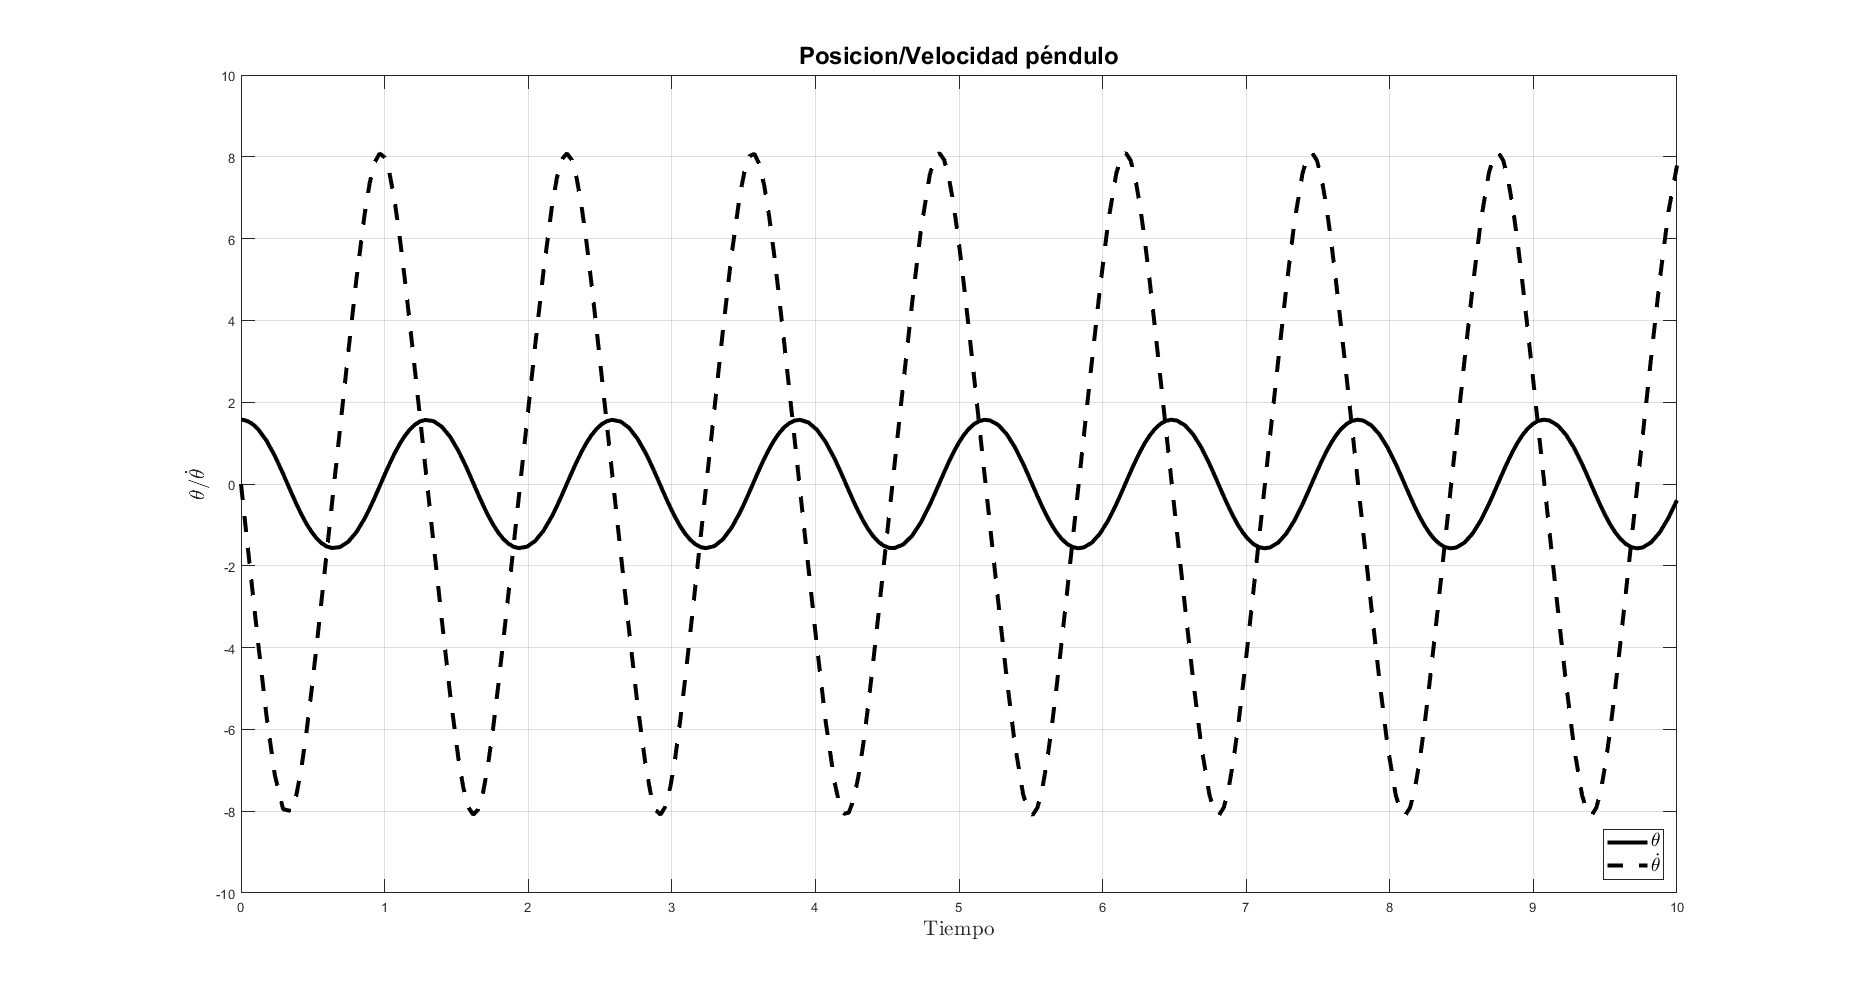
\includegraphics[scale=0.2]{../Report/img/PosVelNF.png}
%  % fasependulox2.png: 1853x1003 px, 96dpi, 49.02x26.53 cm, bb=0 0 1390 752
%  \caption{Comportamiento de $\theta(t)$ y $\dot{\theta}(t)$ en el tiempo sin fricción.}
%  \label{fig: time plot theta dtheta no friction}
% \end{figure}
% 
% \end{frame}
% 
% 
% \begin{frame}{Caso sin fricción}
% \begin{figure}[hb!]
%  \centering 
%  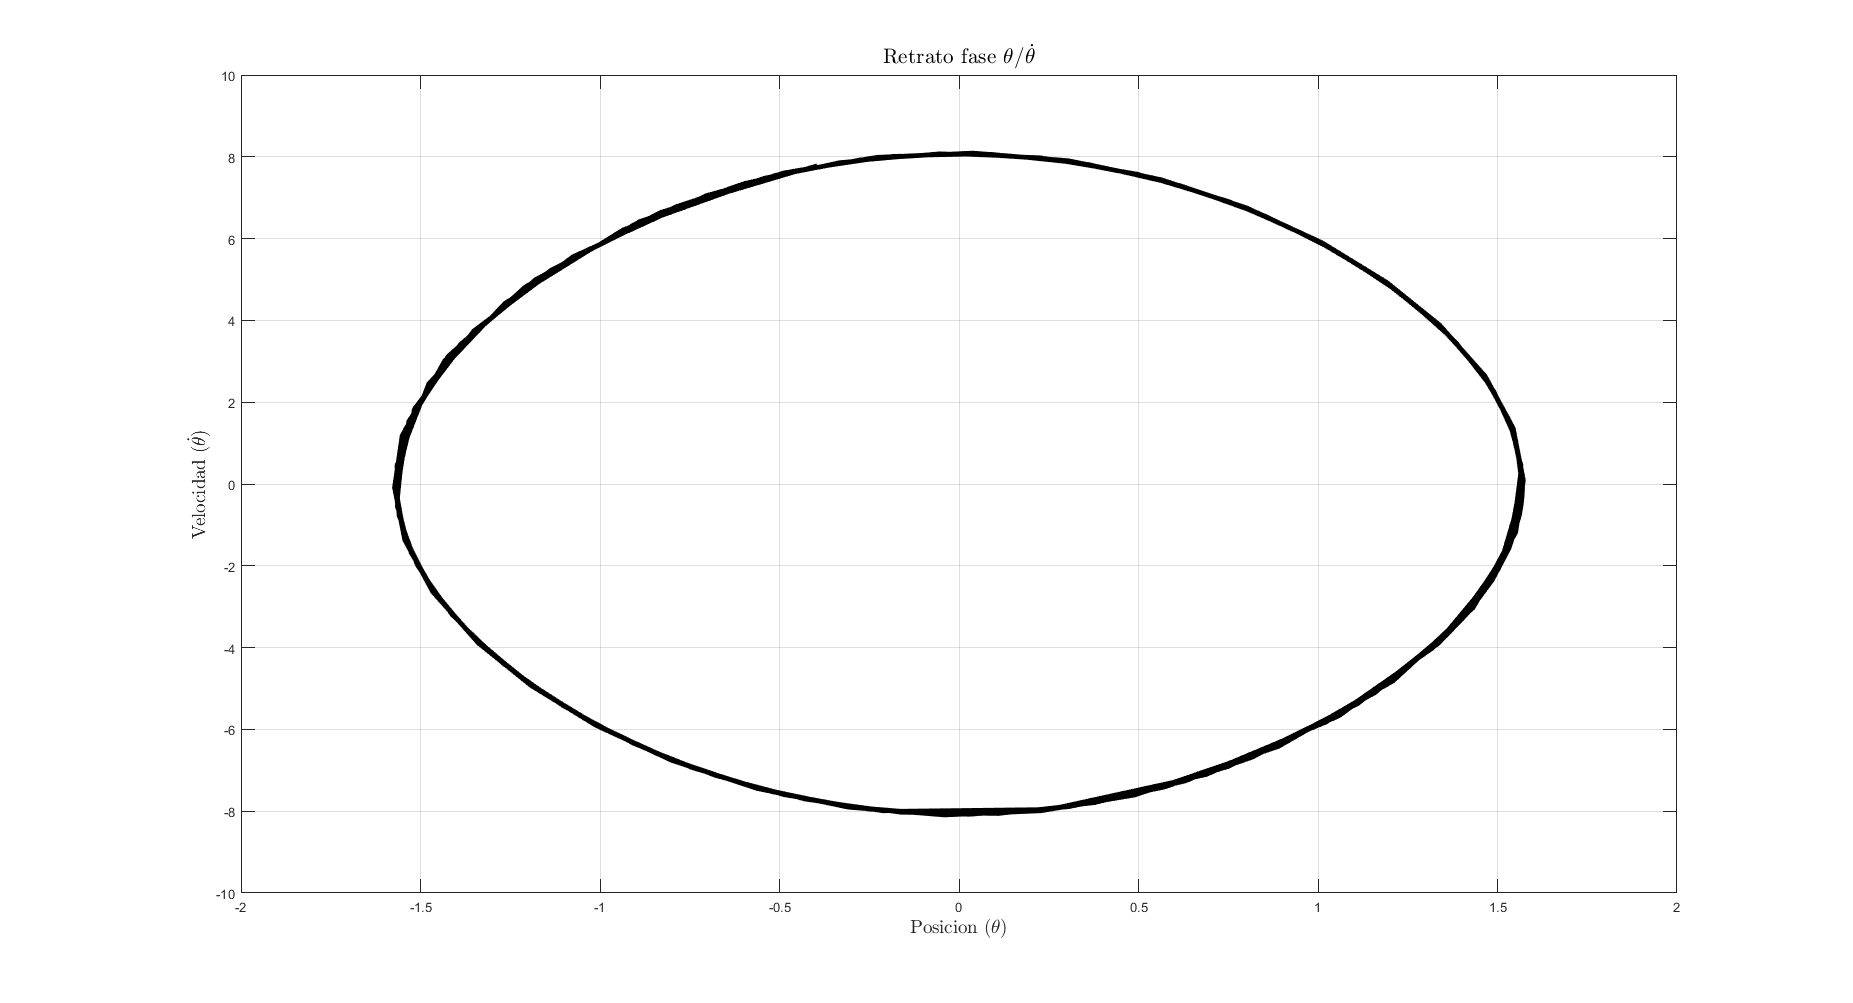
\includegraphics[scale=0.2]{../Report/img/faseNF.png}
%  % fasependulox2.png: 1853x1003 px, 96dpi, 49.02x26.53 cm, bb=0 0 1390 752
% \caption{Diagrama de fase de $\theta(t)$ y $\dot{\theta}(t)$ sin fricción.}
%  \label{fig: phase plot theta no friction}
% \end{figure}
% 
% \end{frame}
% 
% 
% \begin{frame}{Caso con fricción}
% \begin{figure}[hb!]
%  \centering 
%  \includegraphics[scale=0.2]{../Report/img/PosVelF.png}
%  % fasependulox2.png: 1853x1003 px, 96dpi, 49.02x26.53 cm, bb=0 0 1390 752
%  \caption{Comportamiento de $\theta(t)$ y $\dot{\theta}(t)$ en el tiempo.}
%  \label{fig: time plot theta dtheta friction}
% \end{figure}
% 
% \end{frame}
% 
% \begin{frame}{Caso con fricción}
% \begin{figure}[hb!]
%  \centering 
%  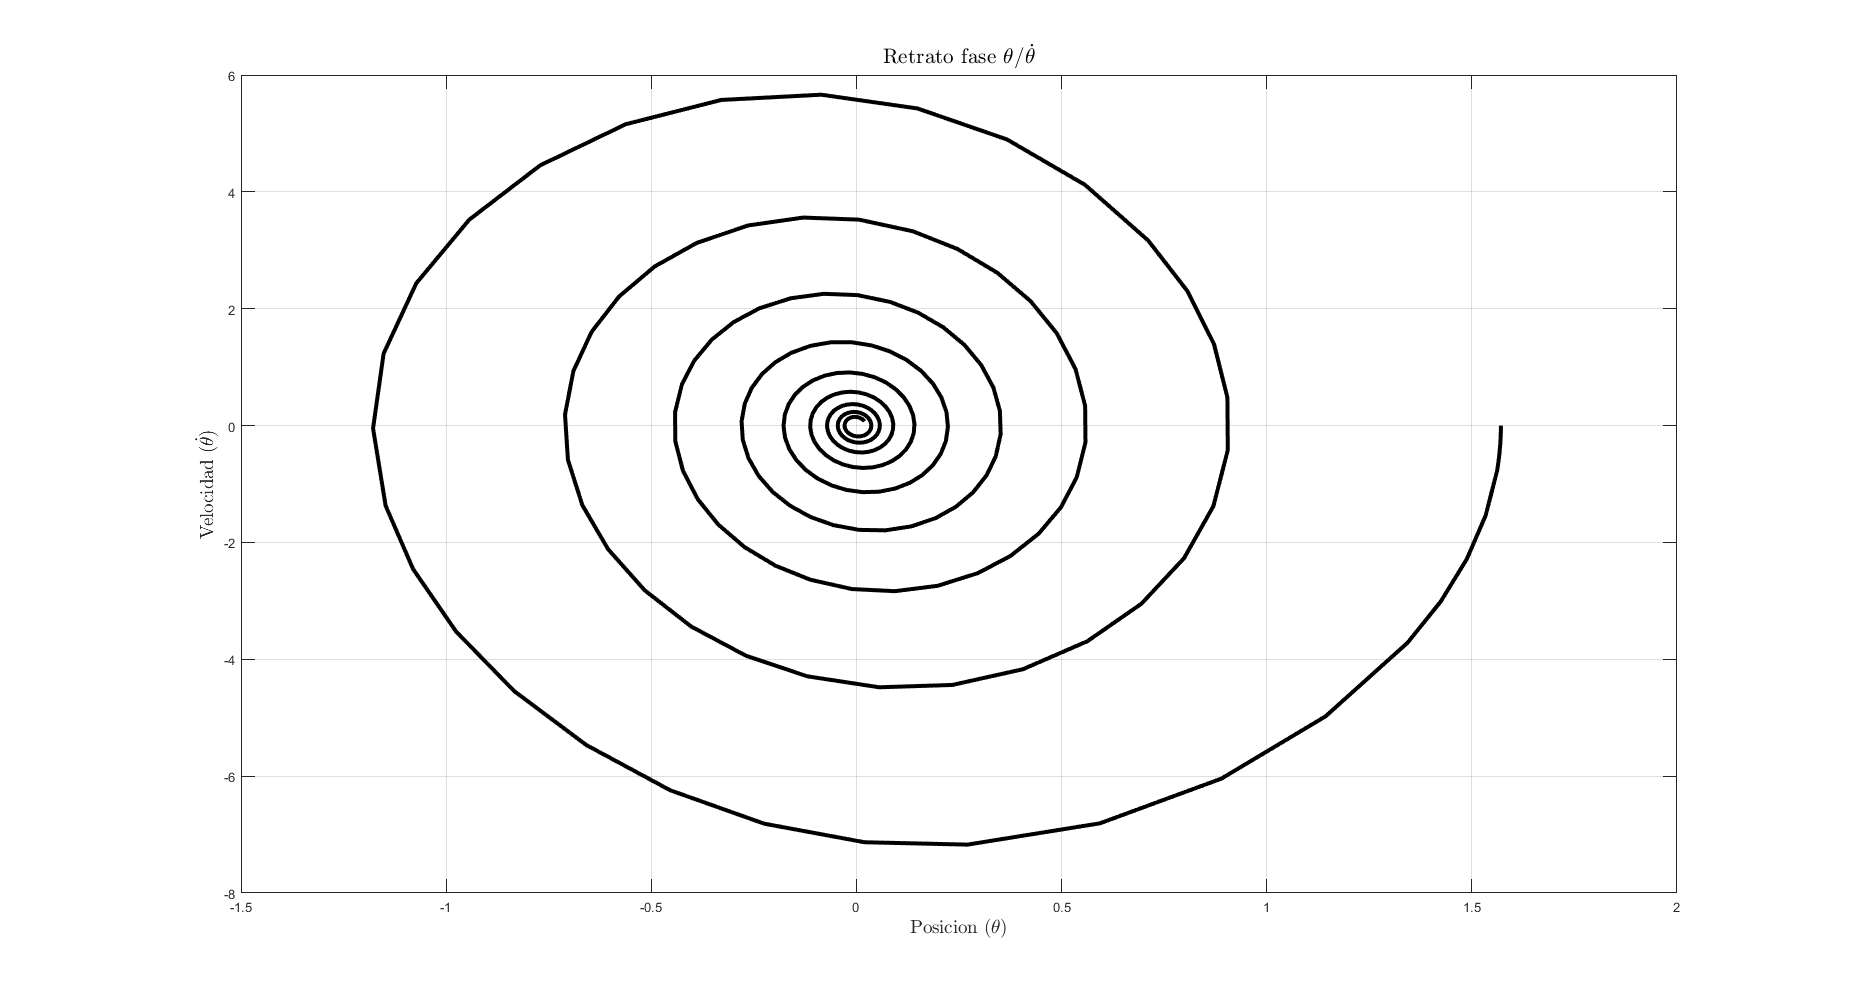
\includegraphics[scale=0.2]{../Report/img/faseF.png}
%  % fasependulox2.png: 1853x1003 px, 96dpi, 49.02x26.53 cm, bb=0 0 1390 752
% \caption{Diagrama de fase de $\theta(t)$ y $\dot{\theta}(t)$.}
%  \label{fig: phase plot theta friction}
% \end{figure}
% 
% \end{frame}
% 
% 
% \section{Modelo físico}
% \subsection{LEGO Mindstorms}
% 
% \begin{frame}{Mediciones}
%  \begin{figure}[hb!]
%  \centering
%  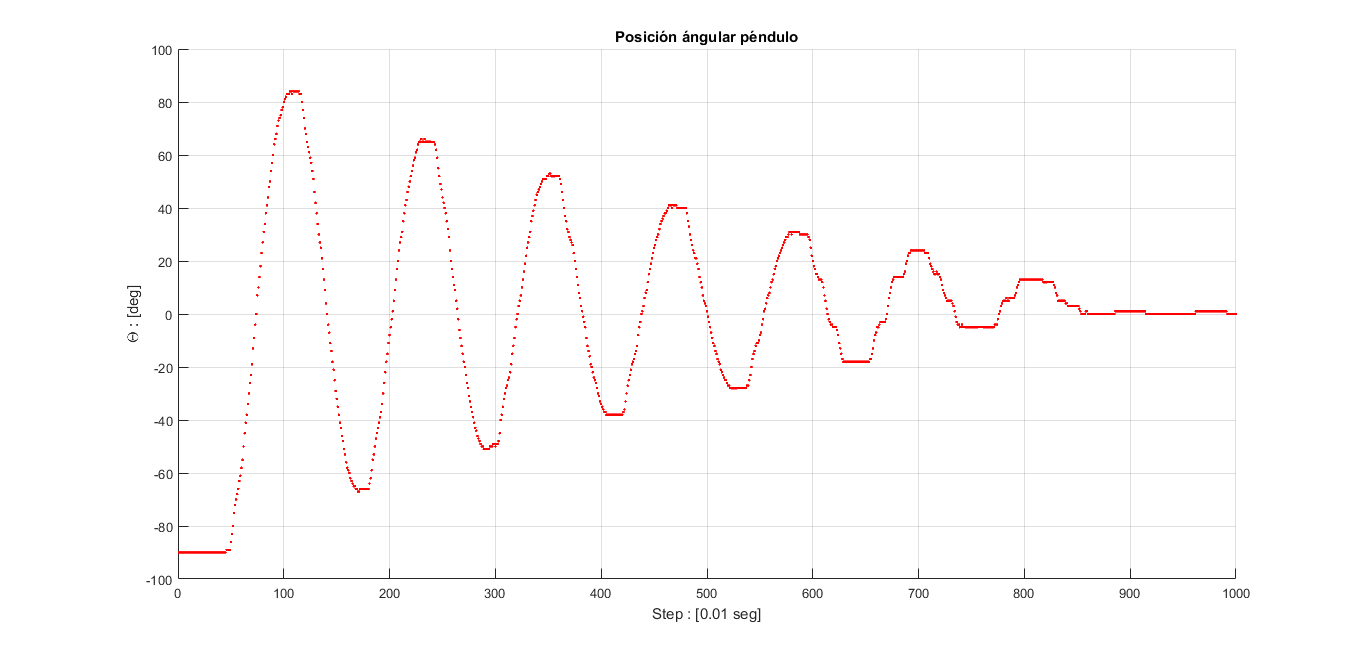
\includegraphics[scale=0.3]{../Mindstorms/Pendulin2.png}
%  % Pendulin2_bw.png: 1157x625 px, 96dpi, 30.61x16.53 cm, bb=0 0 868 469
%  \caption{Mediciones de $\theta$.}
%  \label{fig: mindstorms theta}
% \end{figure}
% \end{frame}
% 
% 
% \begin{frame}{Análisis de video}
%  \begin{figure}[h]
%  \centering
%  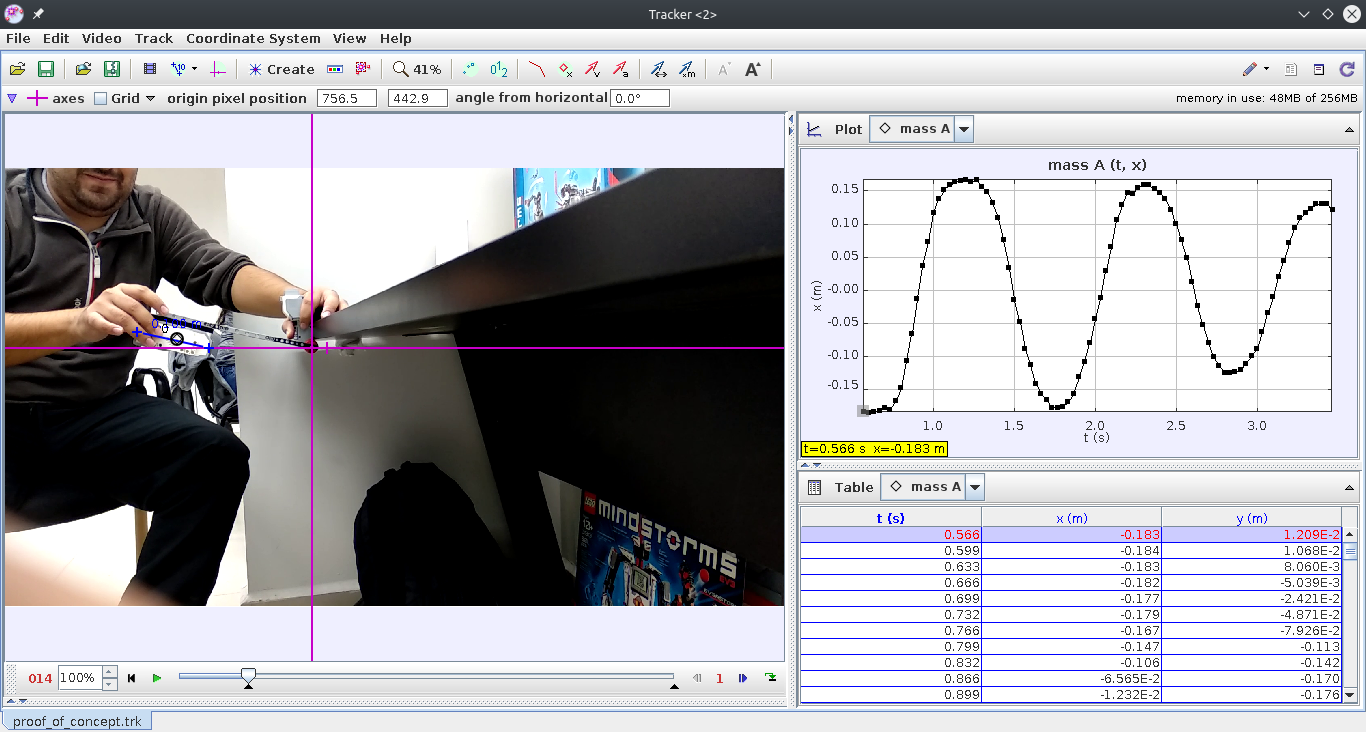
\includegraphics[scale=0.2]{../Report/img/tracker_poc.png}
%  % tracker_poc.png: 1366x732 px, 96dpi, 36.14x19.37 cm, bb=0 0 1024 549
%  \caption{Análisis de movimiento - Prueba de concepto.}
%  \label{fig: tracker main window}
% \end{figure}
% 
% \end{frame}
% 
% \begin{frame}{Análisis de video}
%  \begin{figure}[h]
%  \centering
%  \includegraphics[scale=0.2]{../Report/img/tracker_poc_phasediagram_x_vx.png}
%  % tracker_poc_phasediagram_x_vx.png: 844x585 px, 72dpi, 29.78x20.64 cm, bb=0 0 844 585
%  \caption{Diagrama de fase de $x$ y $\dot{x}$ del modelo físico.}
%  \label{fig: tracker phase diagram x vx}
% \end{figure}
% 
% \end{frame}
% 
% \begin{frame}{Análisis de video}
%  \begin{figure}[h]
%  \centering
%  \includegraphics[scale=0.2]{../Report/img/tracker_poc_phasediagram_y_vy.png}
%  % tracker_poc_phasediagram_x_vx.png: 844x585 px, 72dpi, 29.78x20.64 cm, bb=0 0 844 585
%  \caption{Diagrama de fase de $y$ y $\dot{y}$ del modelo físico.}
%  \label{fig: tracker phase diagram y vy}
% \end{figure}
% 
% \end{frame}
% 
% \begin{frame}{}
%  
% \end{frame}


\end{document}


